\documentclass{beamer}
\usetheme{Madrid}

\title{Physics Research Showcase}
\subtitle{Numerical solutions to the DGLAP equations}
\author{Casey Hampson}
\date{18 April, 2025}


%math stuff
\usepackage{amsmath}
\usepackage{amssymb}
\usepackage{siunitx}
\usepackage{mathtools}
\usepackage{esdiff}
\usepackage{esint}
\usepackage{bm}
\usepackage{tikz-feynman}

\newcommand{\dd}{\mathrm{d}}
\newcommand{\vv}[1]{\mathbf{\bm{#1}}}


\begin{document}
\frame{\titlepage}

% add NSF logo and 
% National Science Foundation (NSF) Grant: PHY-2412071.
% along with Dr.Guzzi's name to the title page



\begin{frame}
  \frametitle{Introduction}

  \begin{itemize}
  \item High-energy physicists are tasked with determining the behavior of the universe on the smallest possible scales.
  \item The particle accelerator located at CERN in Geneva, Switzerland provides us with a unique opportunity to answer some of our most important questions.
  \item The LHC accelerates protons to nearly the speed of light along a 16.8 mile ring and collides them.
  \item In a high energy proton-proton collision, protons break down many additional particles are produced in the final state.
  \end{itemize}

  \begin{figure}
    \centering
    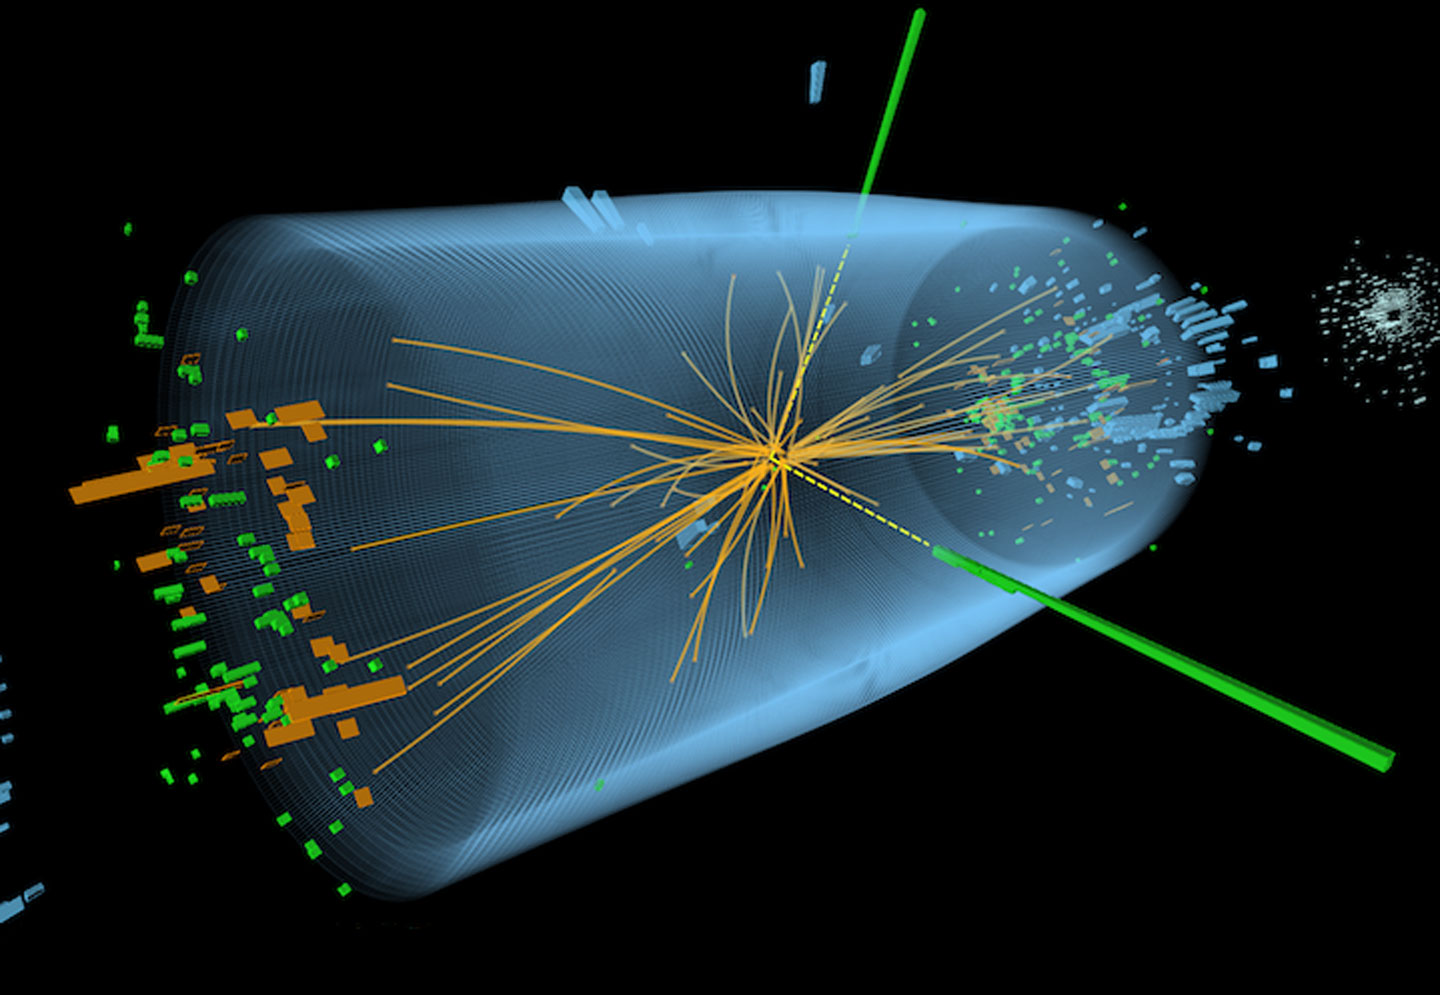
\includegraphics[width=0.35\linewidth]{./gfx/lhc.jpg}
    %\caption{Simulated scattering event at the LHC.}
    %\label{fig:lhc}
  \end{figure}
  
\end{frame}


\begin{frame}
  \frametitle{Photos from Summer 2024 REU at CERN}

  \begin{figure}
    \centering
    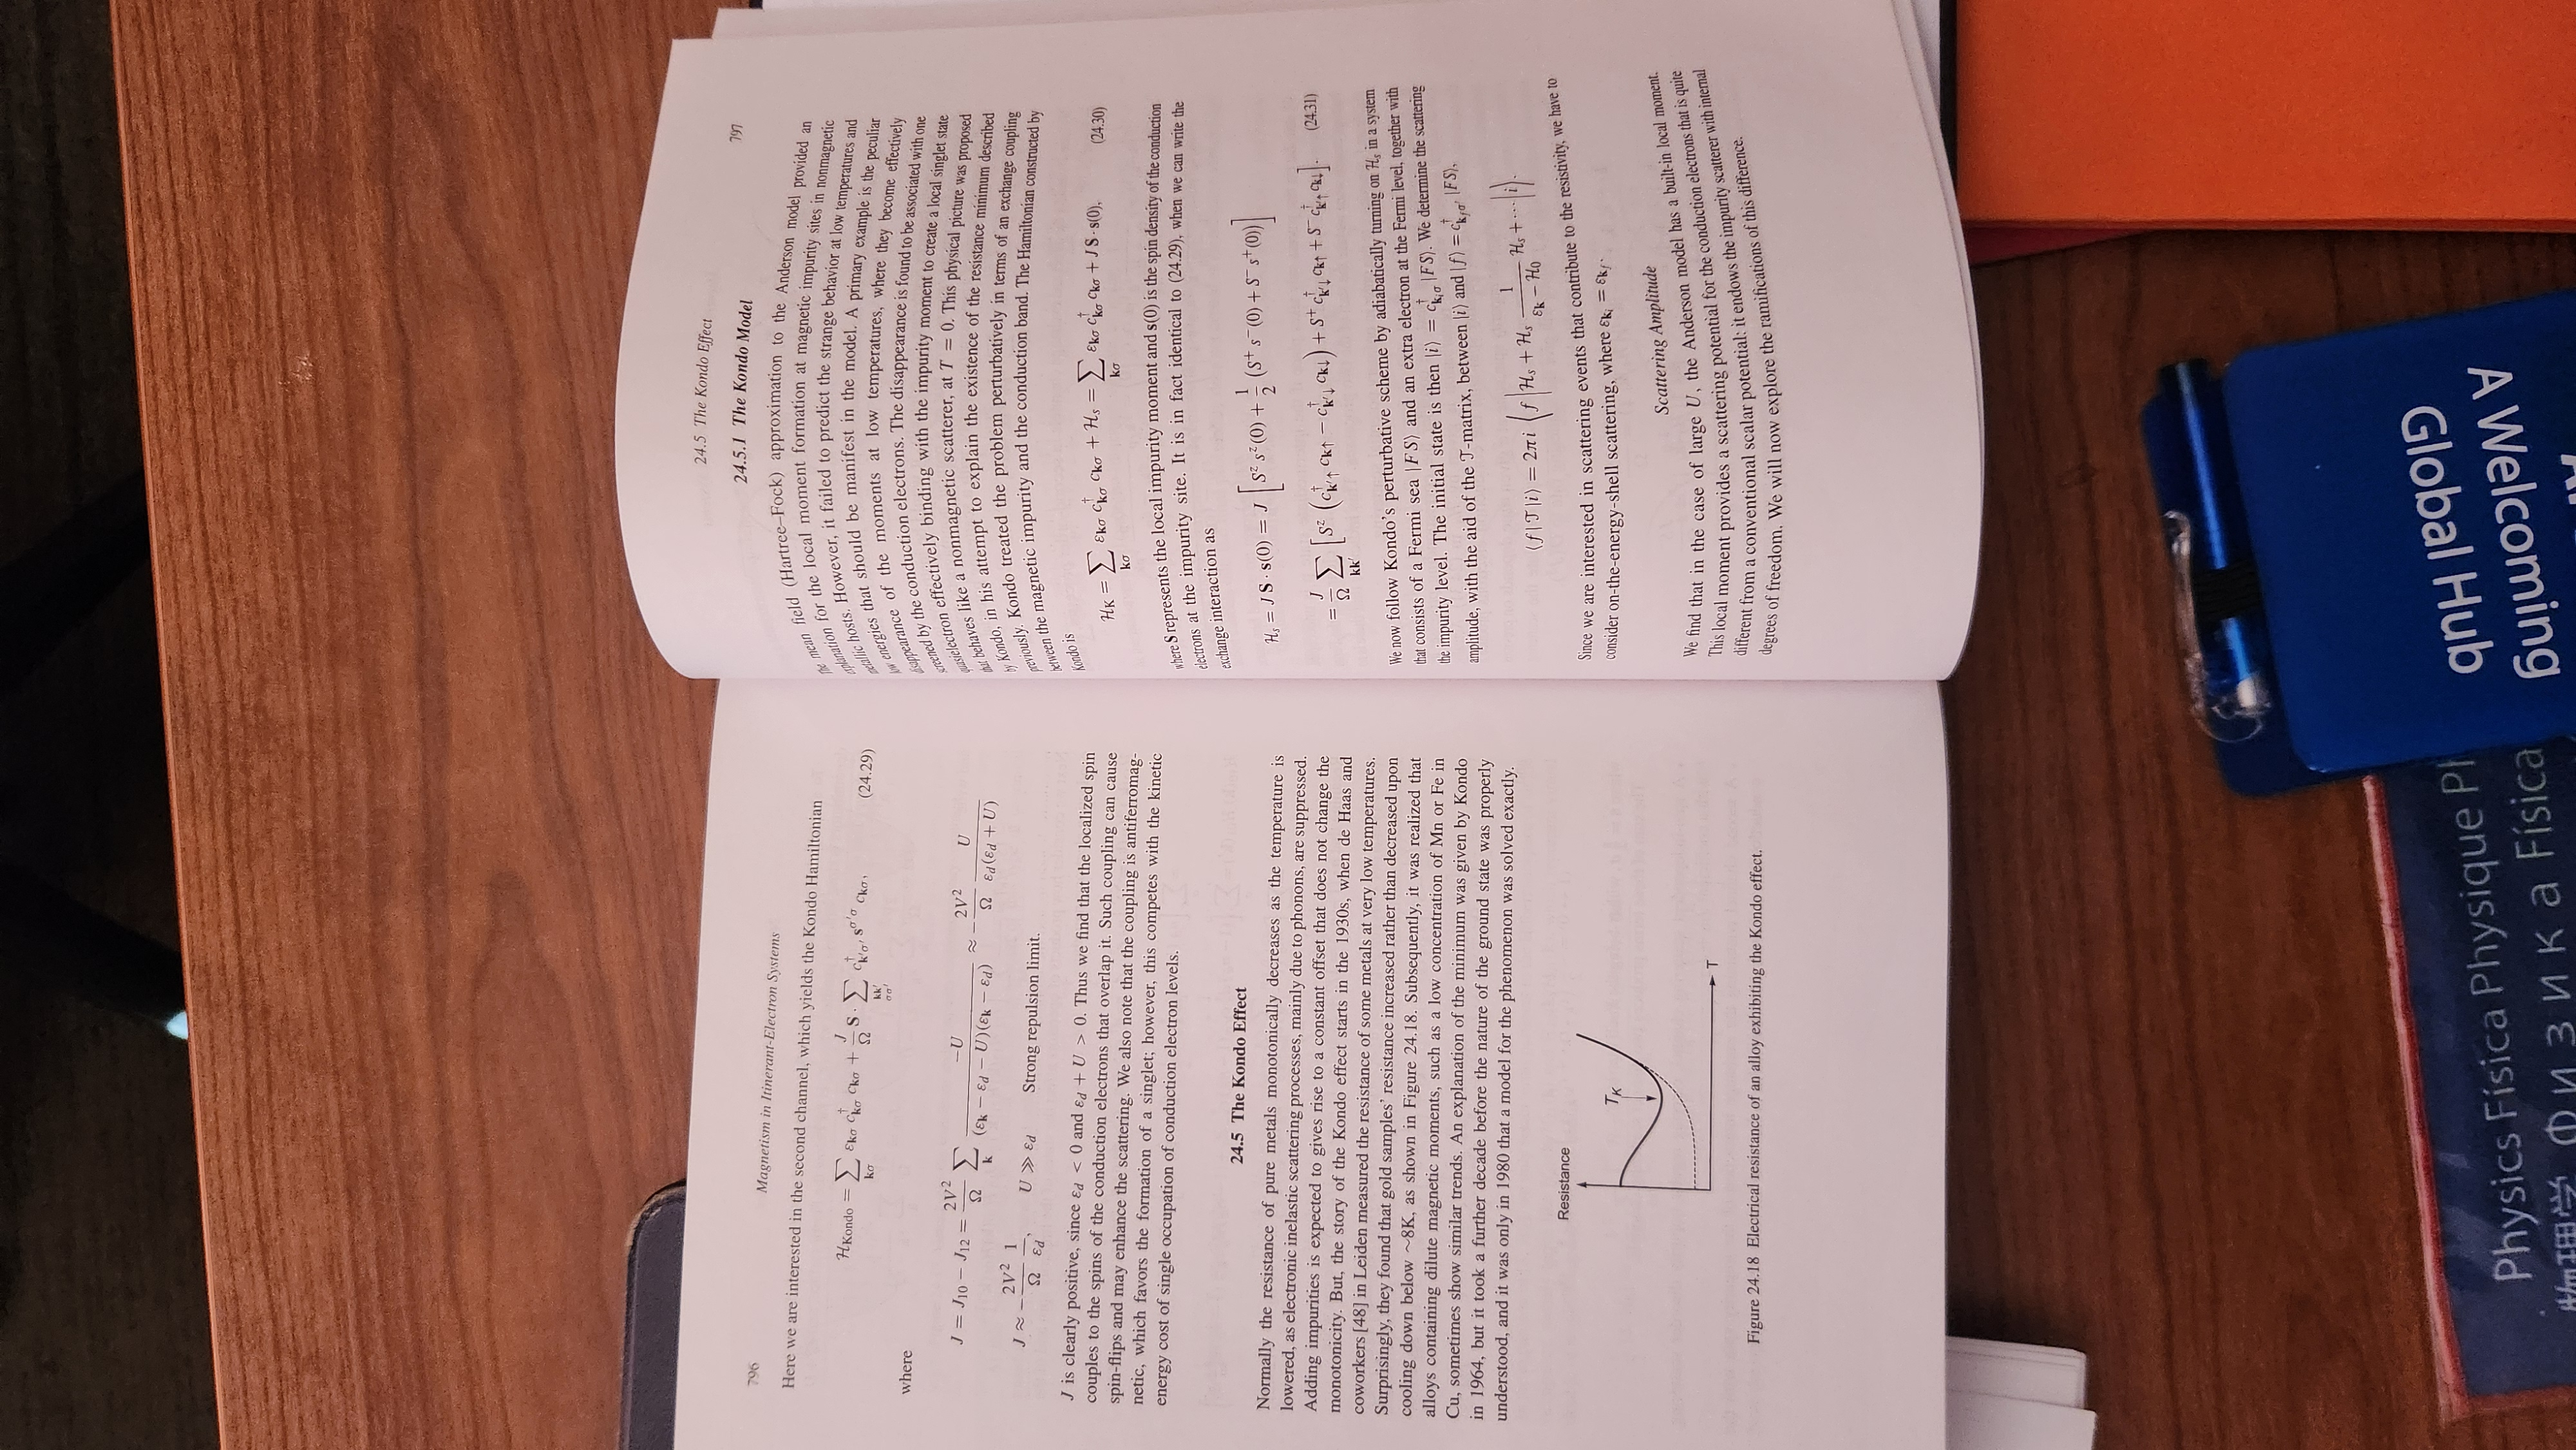
\includegraphics[width=0.6\linewidth]{./gfx/cern/1.jpg}
    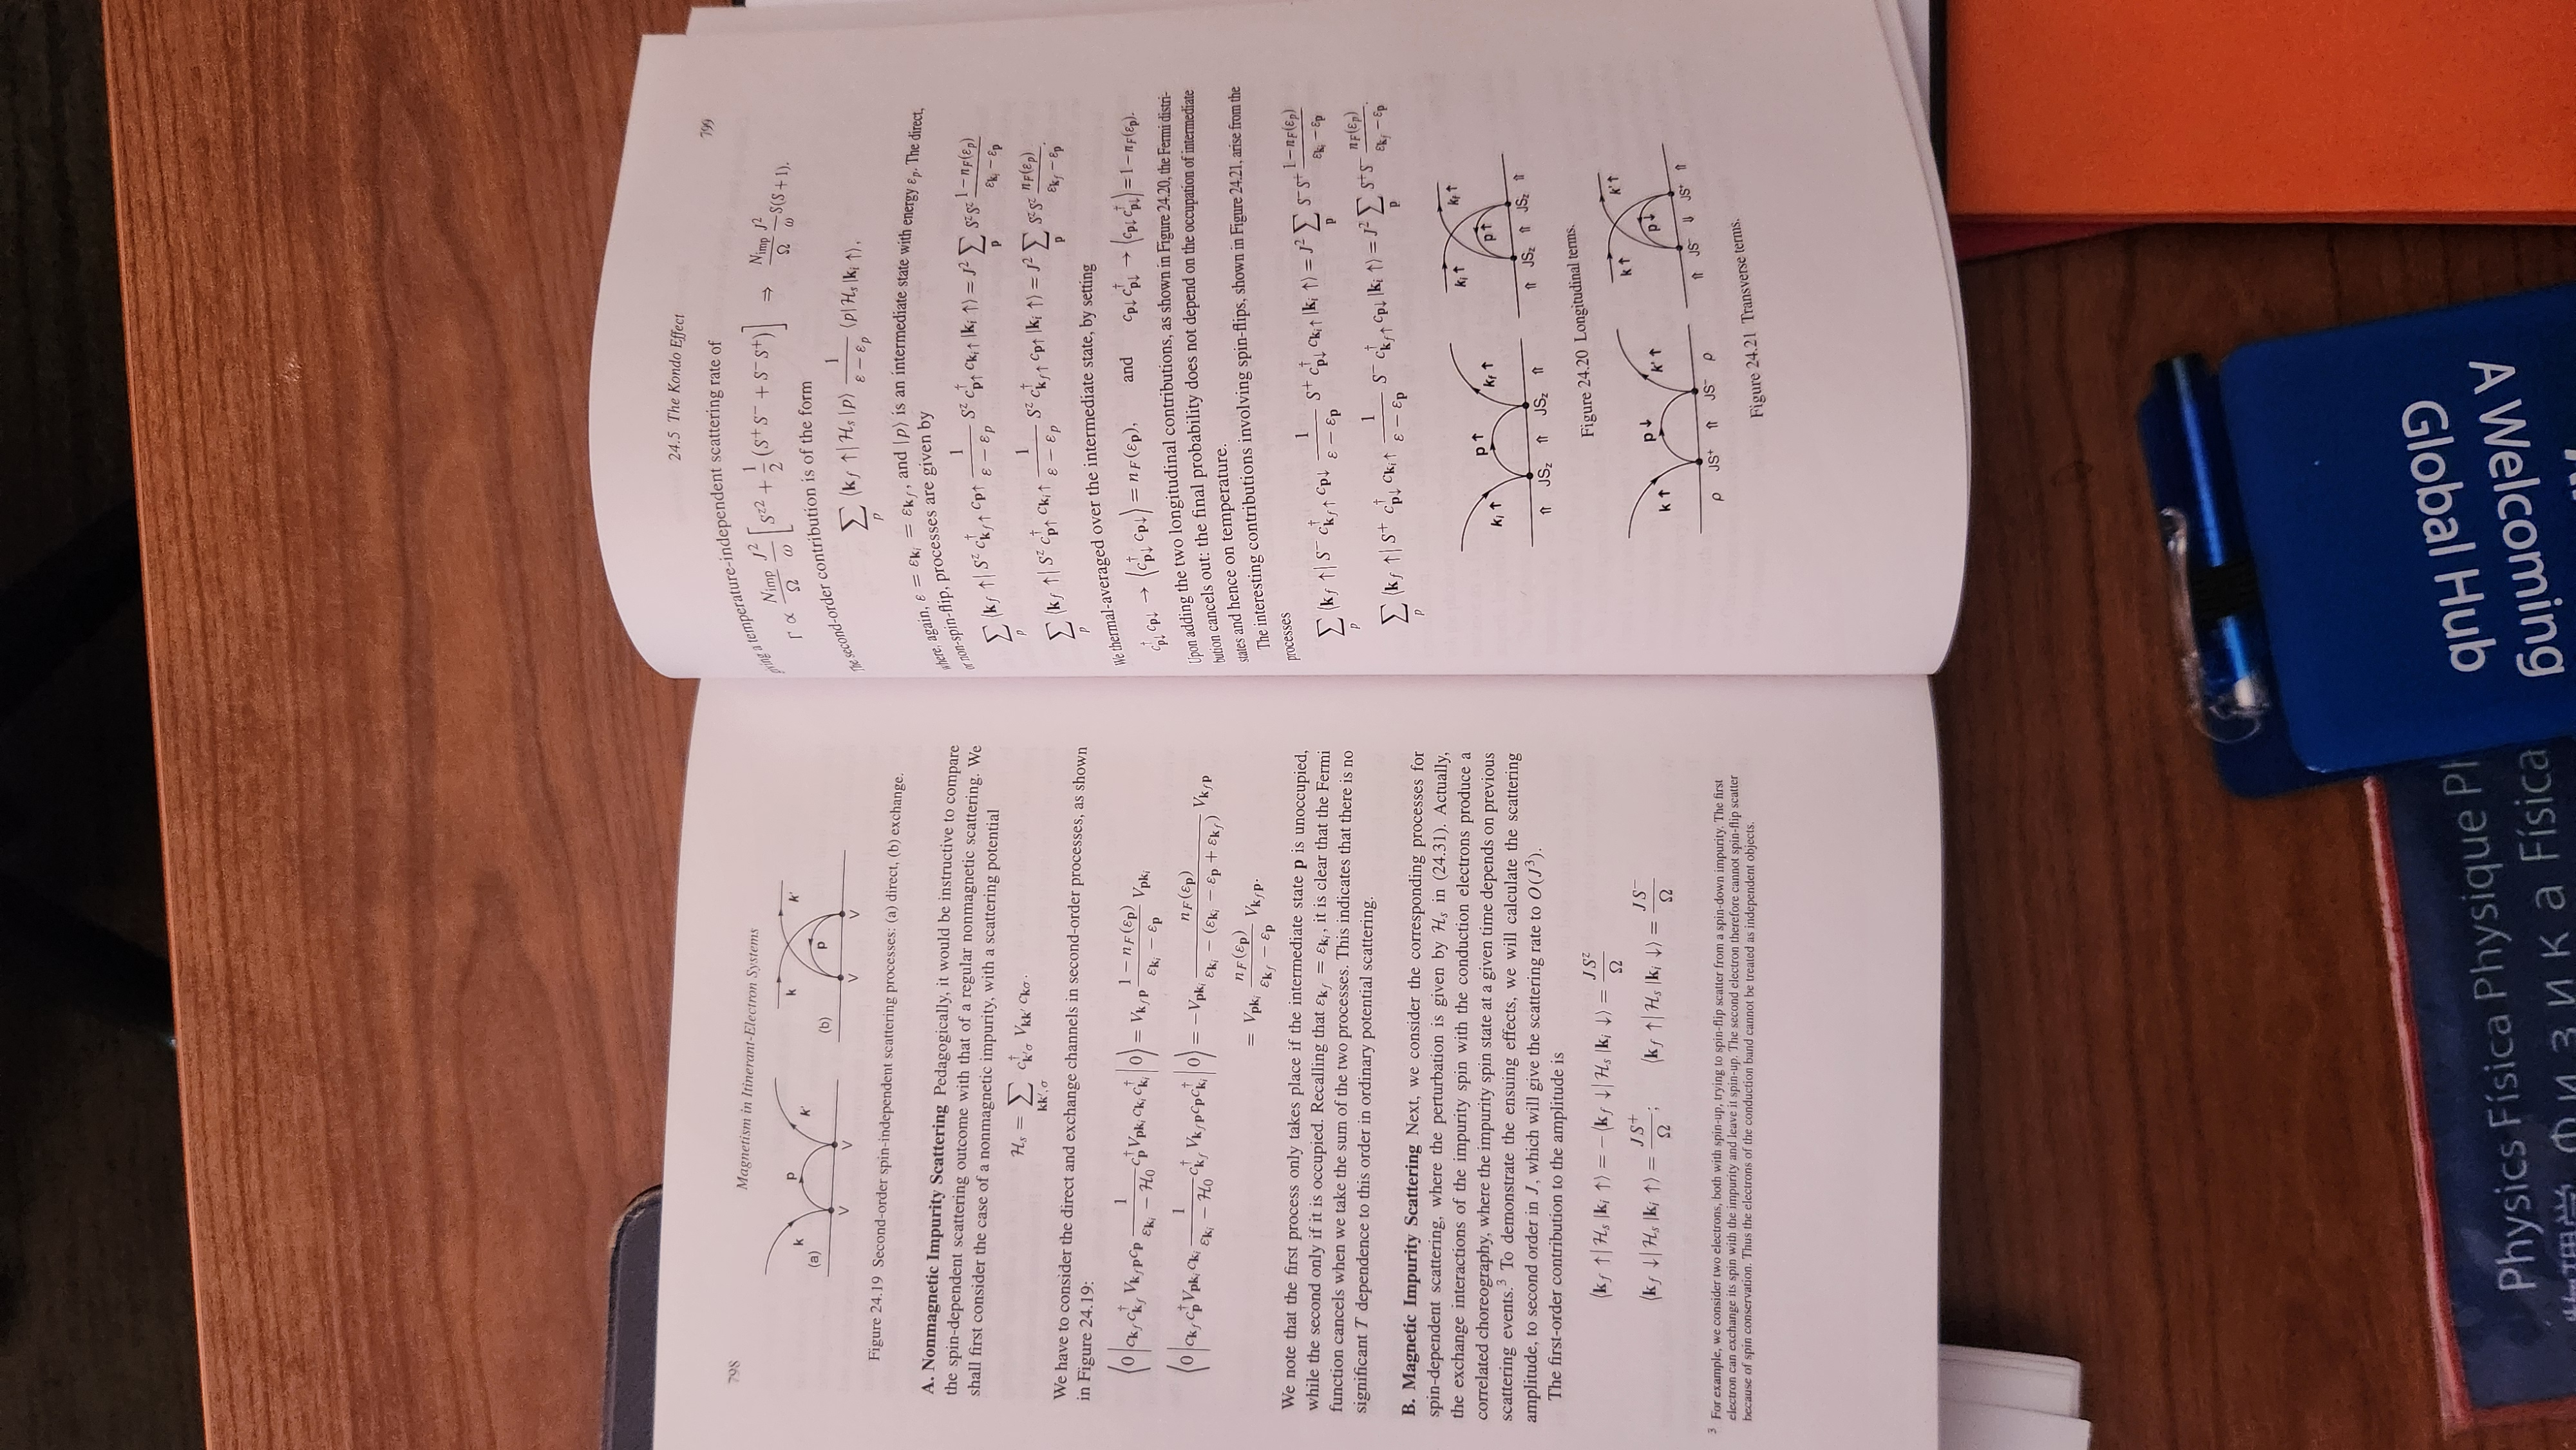
\includegraphics[width=0.6\linewidth]{./gfx/cern/2.jpg}
  \end{figure}
  
\end{frame}

\begin{frame}
  \frametitle{Photos from Summer 2024 REU at CERN}

  \begin{figure}
    \centering
    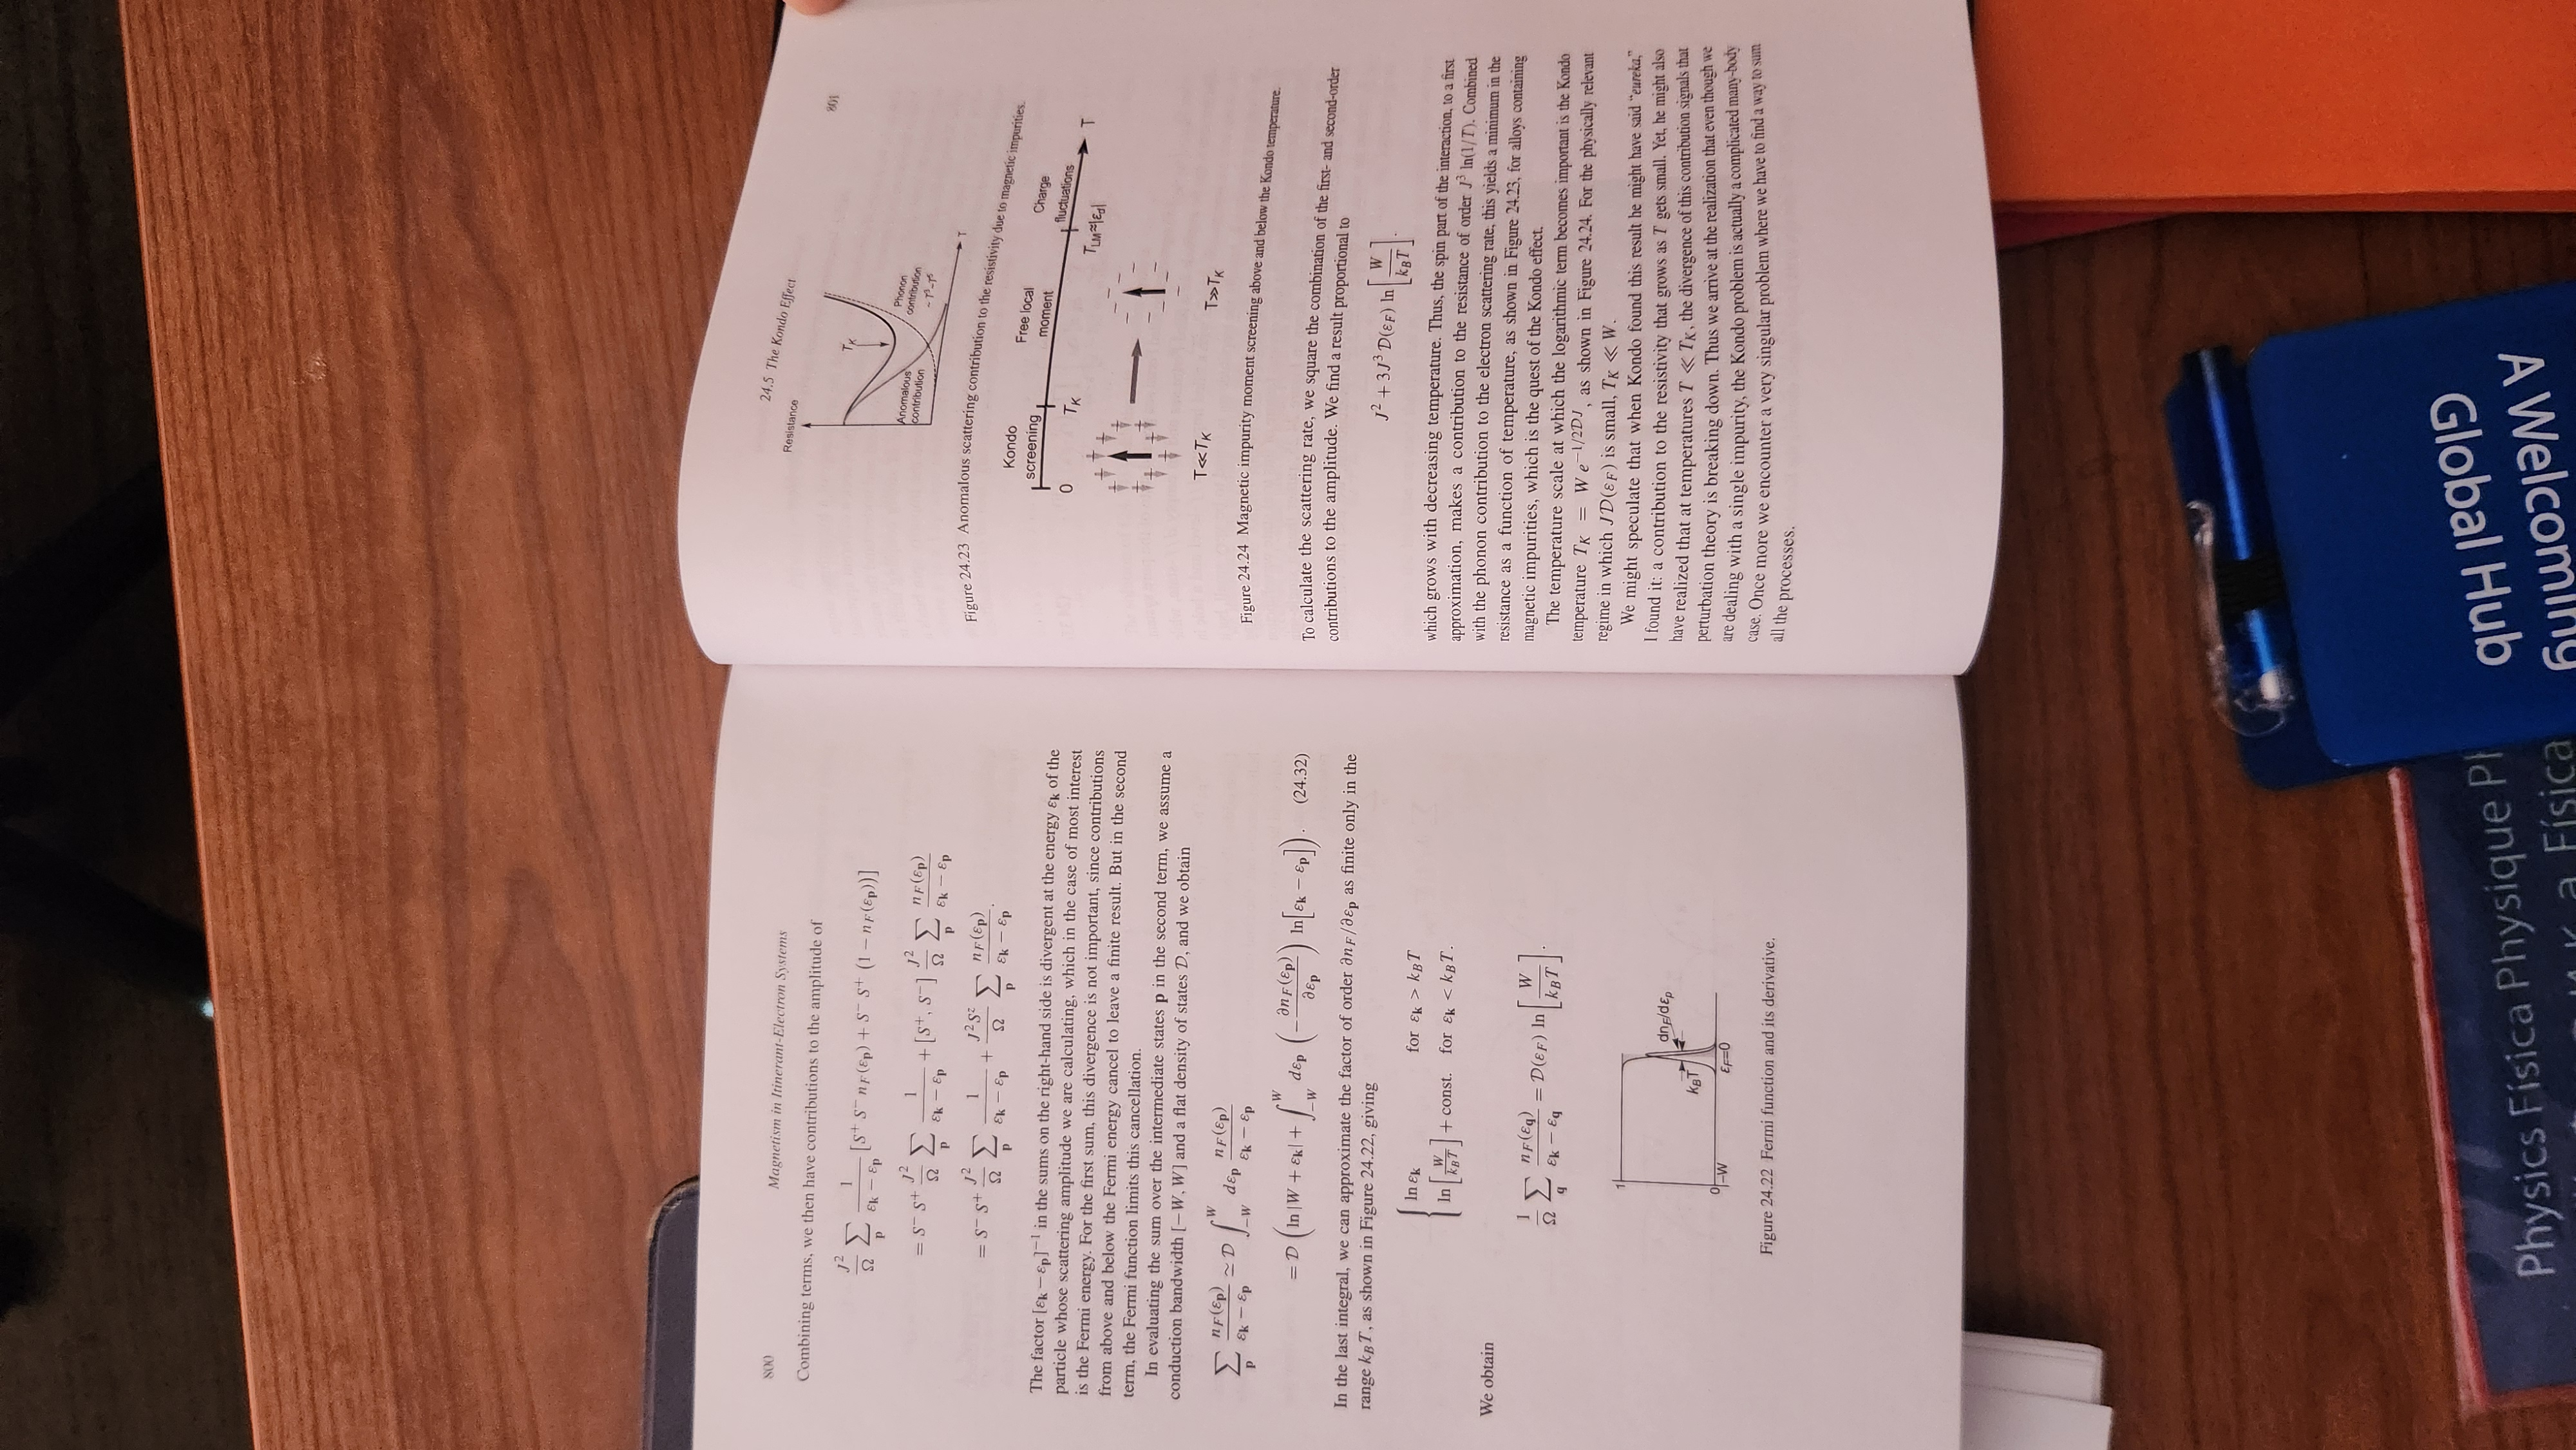
\includegraphics[width=0.6\linewidth]{./gfx/cern/3.jpg}
    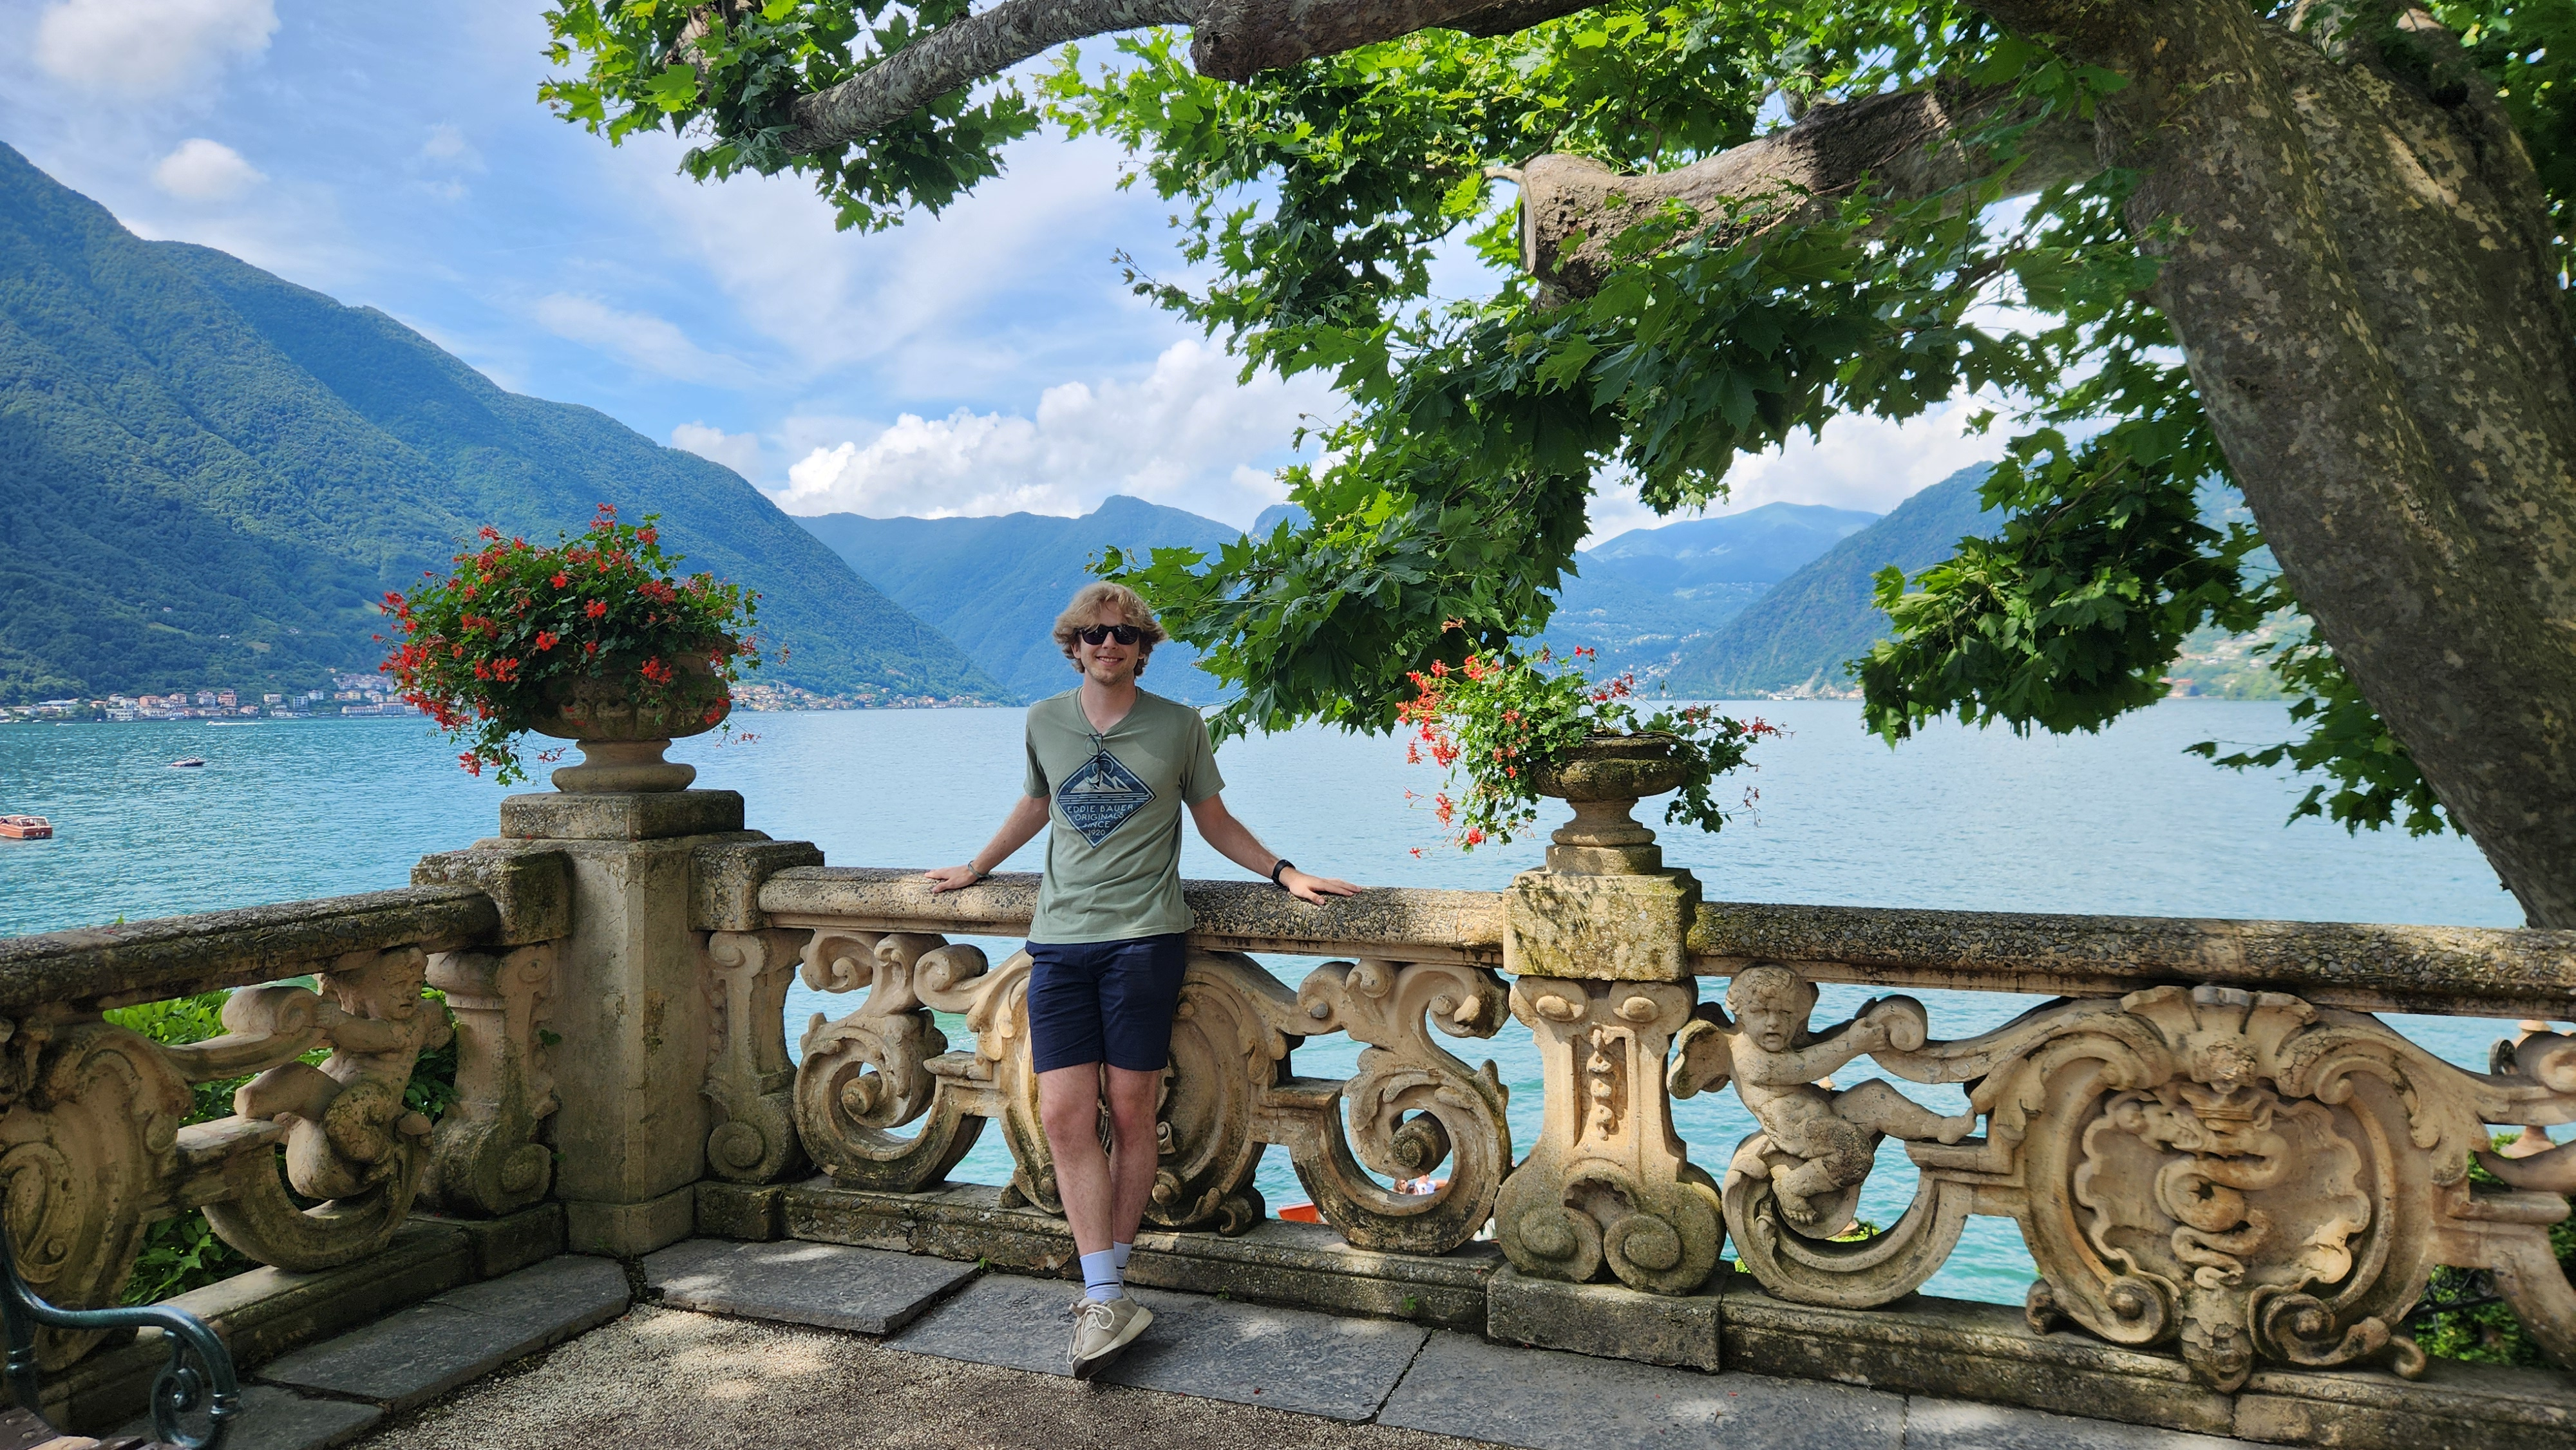
\includegraphics[width=0.6\linewidth]{./gfx/cern/4.jpg}
  \end{figure}
  
\end{frame}


\begin{frame}
\frametitle{Parton Distribution Functions}

\begin{itemize}
\item Parton Distribution Functions (PDFs) are experimentally determined distributions that give probabilities of finding partons (i.e. quarks and gluons) with momentum fraction $x$ within the proton at an energy scale $Q$.
\end{itemize}

\begin{figure}
  \centering
  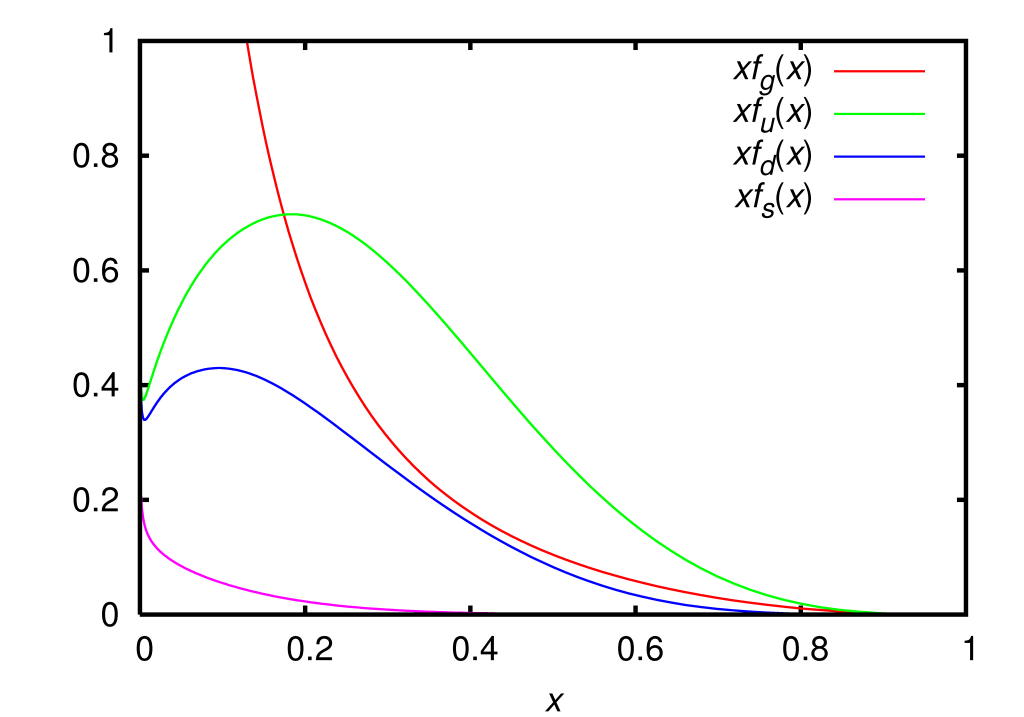
\includegraphics[width=0.4\linewidth]{./gfx/pdfs.png}
  \caption{Parton distributions for the first few light quark flavors and the gluon from the CTEQ group, evaluated at $\qty{2}{\giga\electronvolt}$.}
  \label{fig:pdfs}
\end{figure}

\end{frame}


\begin{frame}
  \frametitle{DGLAP Evolution Equations}

  \begin{itemize}
  \item Unfortunately, PDFs are not able to be calculated from first principles.
  \item We can, however, determine how they evolve with energy via the DGLAP (Dokshitzer-Gribov-Lipatov-Altarelli-Parisi) equations.
  \item These are a set of integro-differential equations that go like:
  \end{itemize}

  \begin{equation}
    \frac{\partial}{\partial \ln Q^2} = P(x, \alpha_s(Q^2)) \otimes f(x, Q^2),
  \end{equation}

  where $f$ is the PDF, $\alpha_s$ is the strong coupling constant, and $P$ is the \textit{splitting function}, which roughly corresponds to probabilities for quarks to emit gluons and vice versa. The $\otimes$ corresponds to a convolution, defined like so:

  \begin{equation}
    [a \otimes b](x) = \int_x^1 \frac{\dd y}{y} a\left( \frac{x}{y} \right) b(y) = \int_x^1 \frac{\dd y}{y} a(y) b\left( \frac{x}{y} \right).
  \end{equation}

\end{frame}


% for this slide, remove most of the stuff and simply mention other methods
% which have some pros and cons, but we want to remain in x since that's real life space
% and we keep the analytical/mathematical structure
\begin{frame}
  \frametitle{Solutions to the DGLAP Equations}

  \begin{itemize}
  \item Solutions are particularly challenging due to the convolution appearing on the R.H.S.
  \item One main solution is moving to Mellin space:
  \end{itemize}

  \begin{equation}
    a(N) = \int_0^1 \dd x \; x^{N-1}a(x)
  \end{equation}

  which turns a convolution into a normal product:

  \begin{equation}
    [a \otimes b](N) = a(N) \cdot b(N).
  \end{equation}

  \begin{itemize}
  \item This, however, incurs the cost of transforming to and from $x$-space and Mellin space. It also loses the main mathematical and physical structure of the equations, which is something we want to keep.
  \end{itemize}
\end{frame}


\begin{frame}
  \frametitle{The Non-singlet Case}

  \begin{itemize}
  \item There are two classes of solutions called ``singlet'' and ``non-singlet.'' The singlet case involves matrices, and the non-singlet involves scalars. The non-singlet case is therefore much more simple.
  \item For this case at Leading Order (LO), one particular ansatz that evolves the PDF $f$ from an initial scale $Q_0^2$ to a final scale $Q^2$ is given by:
  \end{itemize}

  \begin{equation}
    f(x, Q^2) = \sum_{n=0}^{\infty} \frac{A_n(x)}{n!} \ln^n\left( \frac{a_s(Q^2)}{a_s(Q_0^2)} \right),
  \end{equation}

  \begin{itemize}
  \item The $A_n(x)$s satisfy a recursion relation:
  \end{itemize}

  \begin{equation}
    A_{n+1}(x) = - \frac{2}{\beta_0}[P^{(0)} \otimes A_n] (x).
  \end{equation}
\end{frame}


\begin{frame}
  \frametitle{The Non-singlet Case}

  \begin{itemize}
  \item At $NLO$ the ansatz looks roughly the same, but of course with higher order terms 
  \end{itemize}

  \begin{equation}
    f(x, Q^2) = \sum_{n=0}^{\infty}\sum_{s=0}^n \frac{B_n^s(x)}{n!(s-n)!} \ln^n \left( \frac{\alpha_s}{\alpha_0} \right) \ln^{s-n}\left( \frac{4\pi\beta_0 + \alpha_s\beta_1}{4\pi\beta_0 + \alpha_0\beta_1} \right).
  \end{equation}

  \begin{itemize}
  \item The $B_s^n(x)$s will follow more advaned recursion relations as well, i.e. all the $n\neq0$ coefficients first.
  \item Generalizing this to $N^3LO$ is one of our main goals.
  \end{itemize}
\end{frame}


\begin{frame}
  \frametitle{Singlet Ansatz}

  \begin{itemize}
  \item For the singlet case, which are matrices, we consider the solution in Mellin space, which is:
  \end{itemize}

  \begin{equation}
    \vv{f}(N, Q^2) = \left[ 1 + \sum_{k=0}^{\kappa} \alpha_s^k \vv{U}_k \right] \vv{L} \left[ 1 + \sum_{k=0}^{\kappa} \alpha_0^k \vv{U}_k \right]^{-1} \vv{f}(N, Q_0^2).
  \end{equation}

  \begin{itemize}
  \item Here, the $\vv{U}_k$ matrices contain information related to the splitting function which we would keep to only $N^3LO$, but the index $\kappa$ is called a \textit{truncation index}, which in principle we would take to infinity, but practically must keep finite.
  \item In $x$-space, the regular products of these matrices would turn into convolutions. This is currently being tested.
  \end{itemize}
\end{frame}


\begin{frame}
  \frametitle{Current Progress}

  \begin{itemize}
  \item We are currently working with the literature to begin including the most up-to-date version of the $N^3LO$ splitting functions into our code.
  \item The previous \textsc{Candia} code was written in C, but has since been upgraded to C++ with a few minor optimizations. Once the new singlet ansatz and aforementioned splitting function corrections are added we will release the code and call it \textsc{Candia-v2} along with a publication. Time will be spent on improving the algorithm and making further optimizations.
  \item On the next slide are example outputs/plots for the current version of the program.
  \end{itemize}
\end{frame}


\begin{frame}
  \frametitle{Example Outputs}

  \begin{figure}
    \centering
    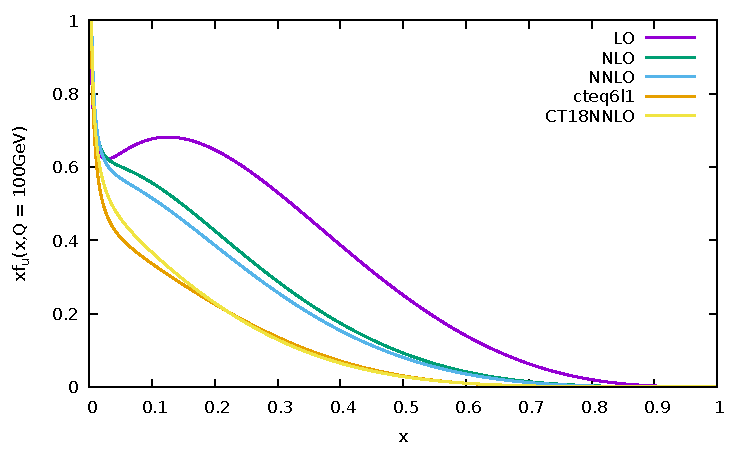
\includegraphics[width=0.51\linewidth]{./gfx/u.pdf}
    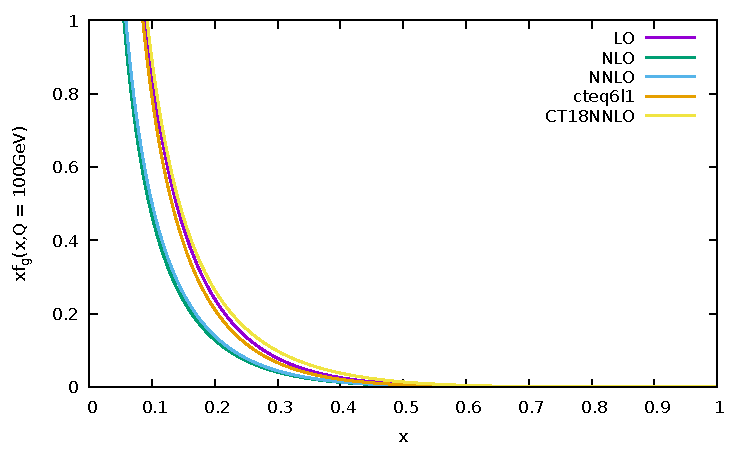
\includegraphics[width=0.51\linewidth]{./gfx/g.pdf}
  \end{figure}
\end{frame}



\end{document}

%%% Local Variables:
%%% mode: LaTeX
%%% TeX-master: t
%%% End:
